\documentclass[aspectratio=43]{beamer}

\usepackage[T2A]{fontenc}
\usepackage[utf8]{inputenc}
\usepackage[english,russian]{babel}
\usepackage{amsmath,amssymb,amsbsy}
\usepackage{graphicx}
\usepackage{booktabs}
\usepackage{microtype}
\usefonttheme[onlymath]{serif}

%% ====================================================================
%%  Тема в стиле защит ФПМИ: красный заголовок в серой рамке,
%%  синие подзаголовки и структура внутри слайда.
%% ====================================================================
\usetheme{default}
\useinnertheme{default}
\useoutertheme{default}
\setbeamertemplate{navigation symbols}{}

\definecolor{titlered}{RGB}{176,42,42}     % красный — заголовки кадров
\definecolor{slideblue}{RGB}{45,55,140}    % синий — структура и подзаголовки
\definecolor{titlebar}{RGB}{236,236,238}   % светло-серая рамка заголовка

%% синий — вся «структура» (маркеры, блоки, акценты)
\setbeamercolor{structure}{fg=slideblue}
\setbeamercolor{title}{fg=titlered}
\setbeamercolor{item}{fg=slideblue}
\setbeamercolor{block title}{fg=slideblue}

%% красный заголовок кадра на серой плашке во всю ширину
\setbeamercolor{frametitle}{fg=titlered,bg=titlebar}
\setbeamerfont{frametitle}{series=\bfseries}
\setbeamerfont{title}{series=\bfseries}

%% собственная боковая граница (без внутренних макросов beamer с @)
\newlength{\fpmargin}\setlength{\fpmargin}{0.8cm}
\setbeamersize{text margin left=\fpmargin,text margin right=\fpmargin}

%% отступ текста заголовка кадра от левого края плашки (больше поля текста,
%% чтобы заголовок не липнул к краю страницы)
\newlength{\fptitleindent}\setlength{\fptitleindent}{1.4cm}

\setbeamertemplate{frametitle}{%
  \nointerlineskip%
  \hspace*{-\fpmargin}%
  \begin{beamercolorbox}[wd=\paperwidth,sep=0pt,%
      leftskip=\fptitleindent,rightskip=\fpmargin]{frametitle}%
    \vskip0.32cm\usebeamerfont{frametitle}\insertframetitle\vskip0.32cm%
  \end{beamercolorbox}%
  \vskip0.4em%
}

%% Нижний колонтитул: номер слайда справа
\setbeamertemplate{footline}{%
  \hfill\usebeamerfont{page number in head/foot}%
  \color{slideblue!70}\scriptsize\insertframenumber\,/\,\inserttotalframenumber\hspace*{1.5em}\vskip4pt%
}

%% Маркеры списков
\setbeamertemplate{itemize item}{\color{slideblue}\textbullet}
\setbeamertemplate{itemize subitem}{\color{slideblue!70}--}
\setbeamertemplate{enumerate item}{\color{slideblue}\insertenumlabel.}

%% Синий подзаголовок-блок внутри слайда («Проблема», «Цель», ...)
\newcommand{\heading}[1]{\smallskip{\color{slideblue}\bfseries #1}\par\nobreak\smallskip}
%% Компактная ссылка на источник
\newcommand{\cit}[1]{{\footnotesize\color{slideblue!75}[#1]}}

\title{Применение методов каузального вывода при анализе зависимостей между оптимизирующими проходами LLVM-компилятора}

\begin{document}

%% ================= Слайд 1: титул =================
\begin{frame}[plain]
  \vfill
  \begin{center}
    \begin{beamercolorbox}[wd=0.92\paperwidth,sep=0.5cm,center,rounded=true]{frametitle}
      \usebeamerfont{title}\large
      Применение методов каузального вывода при анализе
      зависимостей между оптимизирующими проходами
      LLVM-компилятора
    \end{beamercolorbox}

    \vskip1.4em
    Белонин Владимир Викторович\\[0.3em]
    {\small группа М05-002д}\\[0.8em]
    {\small Научный руководитель:\\
      д-р техн. наук, проф. С.\,К.~Дулин\par}
    {\small Научный консультант:\\
      к.ф.-м.н., доцент Н.\,Н.~Ефанов\par}
    \vskip1.2em
    {\footnotesize
      Московский физико-технический институт (НИУ)\\
      Физтех-школа прикладной математики и информатики\\
      Кафедра интеллектуальных систем ФИЦ ИУ РАН\par}
    \vskip1.0em
    {\small Долгопрудный, 2026}
  \end{center}
  \vfill
\end{frame}

%% ================= Слайд 2: введение и цель =================
\begin{frame}{Порядок оптимизирующих проходов: задача и актуальность}
  \small
  \heading{Область}
  Оптимизирующий компилятор применяет десятки проходов; результат зависит не
  только от \emph{выбора} проходов, но и от \textbf{порядка} их применения~---
  это \emph{задача упорядочивания} (phase ordering).

  \heading{Масштаб и востребованность}
  \begin{itemize}
    \item В LLVM более 150 проходов; уже для 33~проходов
      (длина \texttt{-Oz}) число порядков проходов превышает $10^{49}$ \cit{Ashouri, 2018}.
    \item Специализированный порядок заметно улучшает метрику относительно
      \texttt{-O3}/\texttt{-Oz} \cit{Ashouri, 2018}.
  \end{itemize}

  \heading{Цель работы}
  Выявить \textbf{каузальные} зависимости между оптимизирующими проходами LLVM
  и построить интерпретируемые графы их взаимодействий --- с отделением
  причинно-следственных связей от корреляционных --- для понимания структуры
  пространства оптимизаций.
\end{frame}

%% ================= Слайд 3: существующие подходы и проблема =================
\begin{frame}{Существующие подходы и их ограничение}
  \small
  \heading{Три семейства методов}
  \begin{itemize}
    \item \textbf{Итеративная компиляция / автотюнинг} \cit{Fursin, 2011; Ashouri, 2018}~---
      перебор последовательностей; дорого, результат плохо переносится и не
      объясняет структуру пространства.
    \item \textbf{ML-предсказание порядка} \cit{Trofin, 2021; Cummins, 2022}~---
      «чёрный ящик»: предсказывает последовательность, но не даёт интерпретируемых
      зависимостей между проходами.
    \item \textbf{Корреляционные биграммы} \cit{Fursin, 2011}~--- связывают пары
      проходов с выигрышем по совместной встречаемости.
  \end{itemize}

  \heading{Основная проблема}
  Ни один из подходов не отделяет \textbf{причинно-следственную связь} от
  случайной \textbf{корреляции}: совместная встречаемость пары проходов и выигрыша
  не означает, что порядок проходов \emph{вызывает} этот выигрыш. Фиксированные
  \texttt{-O2}/\texttt{-Oz} неоптимальны для конкретных программ.
\end{frame}

%% ================= Слайд 4: базовый метод (корреляционный граф) =================
\begin{frame}{Базовый метод сравнения: корреляционный граф}
  \small
  Граф зависимостей, фактически применяемый на практике \cit{Fursin, 2011}, строится
  по корреляции биграмм проходов с выигрышем относительно \texttt{-Oz}.

  \heading{Построение}
  Для упорядоченной пары $(A,B)$ вводятся биграмма соседства и индикатор выигрыша,
  \[
    T^{(2)}_{AB}=\mathbb{I}[\,A\text{ перед }B\,],\quad
    W=\mathbb{I}[\,M_\pi < M_{\text{Oz}}\,],
  \]
  где $M_\pi$~--- метрика после последовательности $\pi$. Зависимость
  $T^{(2)}_{AB}$ и $W$ проверяется критерием $\chi^2$ по таблице сопряжённости
  $2\times2$ с поправкой на множественность.

  \heading{Недостаток}
  Значимость $\chi^2$ фиксирует лишь \emph{статистическую связь}, а не причину:
  присутствие пары в выигрышных прогонах может быть следствием общих причин.
  \textbf{Корреляция $\ne$ каузация} --- этот разрыв и измеряется в работе.
\end{frame}

%% ================= Слайд 5: предлагаемый подход =================
\begin{frame}{Предлагаемый подход: рандомизированный эксперимент}
  \heading{Идея}
  Если генерировать последовательности проходов \textbf{случайно}, то для любой
  пары $(A,B)$ событие «$A$ раньше $B$» наступает с равной вероятностью и
  \textbf{независимо} от остальных проходов. Случайные перестановки образуют
  \emph{рандомизированный эксперимент}.

  \begin{block}{Утверждение \cit{Imbens, Rubin, 2015}}
    \centering
    В рандомизированном эксперименте средний эффект воздействия $\text{ATE}$
    несмещённо оценивает средний \textbf{каузальный} эффект.
  \end{block}

  \heading{Следствие для задачи}
  Рандомизация \textbf{балансирует конфаундеры} (наличие и позиции прочих проходов,
  длину последовательности) между группами. Поэтому каузальный эффект порядка пары
  оценивается \textbf{напрямую}, без алгоритмов поиска структуры (PC и аналогов).
\end{frame}

%% ================= Слайд 6: формальная постановка =================
\begin{frame}{Формальная постановка и критерий качества}
  \small
  \heading{Переменные (модель потенциальных исходов Неймана--Рубина)}
  \cit{Rubin, 1974}
  \begin{itemize}
    \item \textbf{Воздействие:} $T_{AB}=1$, если $A$ применяется раньше $B$, и
      $T_{AB}=0$ иначе.
    \item \textbf{Исход:} $Y=(M_{\text{raw}}-M_\pi)/M_{\text{raw}}$~--- доля
      устранённых IR-инструкций относительно неоптимизированного кода.
  \end{itemize}

  \heading{Оцениваемая величина}
  Средний эффект порядка пары есть разность условных средних исхода,
  \[
    \text{ATE}(A\!\to\!B)=\mathbb{E}[\,Y\mid T_{AB}=1\,]-\mathbb{E}[\,Y\mid T_{AB}=0\,],
  \]
  которая в силу рандомизации совпадает с каузальным эффектом.

  \heading{Критерий качества ребра графа}
  Ребро $A\!\to\!B$ включается, если эффект \emph{значим} и \emph{практически
  заметен}: $p_{\text{adj}}<0{,}05$ (критерий Уэлча, поправка Бенджамини--Хохберга)
  и $|\text{ATE}|\ge 0{,}005$.
\end{frame}

%% ================= Слайд 7: pipeline метода =================
\begin{frame}{Метод: построение каузального графа}
  \small
  \heading{Этапы (для всех $\binom{89}{2}=3916$ пар проходов)}
  \begin{enumerate}
    \item Оценка $\text{ATE}(A\!\to\!B)$ по прогонам, где присутствуют оба прохода;
      значимость~--- критерий \textbf{Уэлча} \cit{Welch, 1947}.
    \item Поправка на множественную проверку~--- \textbf{Бенджамини--Хохберг}
      (контроль FDR) \cit{Benjamini, Hochberg, 1995}.
    \item Включение ребра по критерию качества; направление~--- по знаку $\text{ATE}$.
  \end{enumerate}

  \heading{Три уровня агрегации}
  \begin{itemize}
    \item \textbf{глобальный}~--- по всем 517 программам (1 граф);
    \item \textbf{по доменным классам}~--- 8 графов (crypto, numeric, multimedia, \dots);
    \item \textbf{по кластерам структуры IR}~--- 6 графов.
  \end{itemize}
  Конвейер выполняется для \textbf{двух формулировок воздействия}: относительный
  порядок и непосредственное соседство.
\end{frame}

%% ================= Слайд 8: группировка программ =================
\begin{frame}{Метод: группировка программ}
  \begin{columns}[T]
    \begin{column}{0.5\textwidth}
      \centering
      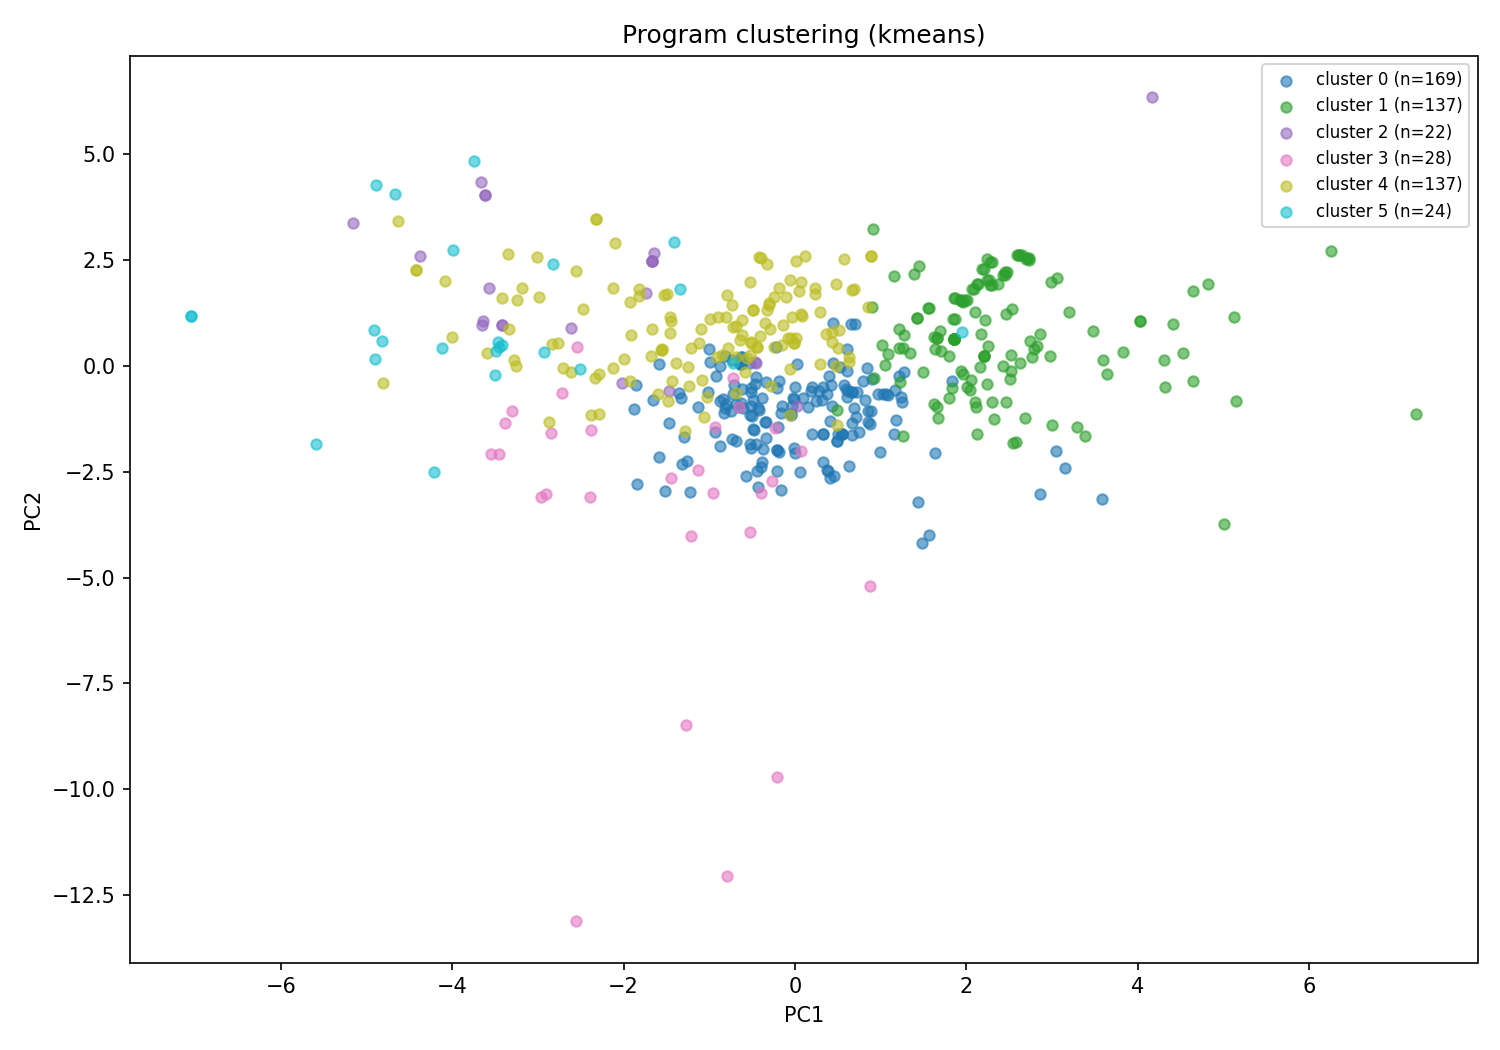
\includegraphics[width=\linewidth]{images/clustering_kmeans.png}\\
      {\footnotesize Кластеризация 517 программ в пространстве признаков IR.}
    \end{column}
    \begin{column}{0.5\textwidth}
      \small
      \heading{Зачем}
      Эффект порядка может различаться по типам программ; графы строятся не только
      глобально.

      \heading{Per-class (по домену)}
      \textbf{8} классов, размеченных вручную по вычислительному домену.

      \heading{Per-cluster (по структуре IR)}
      \textbf{6} кластеров: StandardScaler $\to$ PCA $\to$ KMeans по \textbf{21}
      нормированному признаку IR.

      \medskip
      Группировки слабо совпадают (ARI $=0{,}10$): \textbf{домен $\ne$ структура
      кода}, поэтому используются оба разбиения.
    \end{column}
  \end{columns}
\end{frame}

%% ================= Слайд 9: смещение метрики + CATE =================
\begin{frame}{Метод: смещение метрики и гетерогенность}
  \small
  \heading{Смещение метрики числа IR-инструкций}
  Раздувающий проход на ранней позиции и сокращающий на поздней систематически
  занижают метрику независимо от каузального вклада. Рёбра вида
  «раздуватель $\to$ сократитель» имеют \textbf{двойное смещение}.

  \smallskip
  Их исключение из полного графа (608 рёбер) даёт \textbf{содержательный граф}
  из \textbf{372 рёбер}, на котором ведётся дальнейший анализ.

  \heading{Условный эффект (CATE)}
  Для каждого ребра глобального графа оценивается эффект внутри подгрупп,
  \[
    \text{CATE}_g(A\!\to\!B)=\mathbb{E}[\,Y\mid T_{AB}=1,\,g\,]-\mathbb{E}[\,Y\mid T_{AB}=0,\,g\,],
  \]
  где $g$~--- класс или кластер программ. Смена знака $\text{CATE}$ относительно
  $\text{ATE}$ означает, что ребро \textbf{меняет направление} на подгруппе.
\end{frame}

%% ================= Слайд 10: эксперимент (таблица) =================
\begin{frame}{Вычислительный эксперимент: параметры и данные}
  \begin{columns}[T]
    \begin{column}{0.56\textwidth}
      \footnotesize
      \setlength{\tabcolsep}{4pt}
      \begin{tabular}{@{}ll@{}}
        \toprule
        \textbf{Параметр} & \textbf{Значение}\\
        \midrule
        Компилятор        & LLVM 16, legacy PM\\
        Проходов          & 89\\
        Бенчмарков        & 517\\
        Прогонов/бенчмарк & 10\,000\\
        Всего прогонов    & \textbf{5,17 млн}\\
        Длина $L$         & $\mathcal{U}[10,40]$, без повтор.\\
        Метрика           & число IR-инструкций\\
        Опорные значения  & raw, \texttt{-Oz}\\
        \bottomrule
      \end{tabular}
    \end{column}
    \begin{column}{0.44\textwidth}
      \small
      \heading{Данные}
      517 программ в LLVM IR из двух источников: lac-dcc (cBench, MiBench,
      PolyBench, TSVC и др.) и AnghaBench (функции из GitHub-проектов).

      \heading{Объём}
      Эксперимент: \textbf{19,3 ч} на 6 воркерах; фиксированный seed для
      воспроизводимости.

      \medskip
      Опорное \texttt{-Oz} считается через new PM; raw~--- неоптимизированный код.
    \end{column}
  \end{columns}
\end{frame}

%% ================= Слайд 11: результат — каузальный граф =================
\begin{frame}{Результат: каузальный граф и валидация}
  \begin{columns}[T]
    \begin{column}{0.6\textwidth}
      \centering
      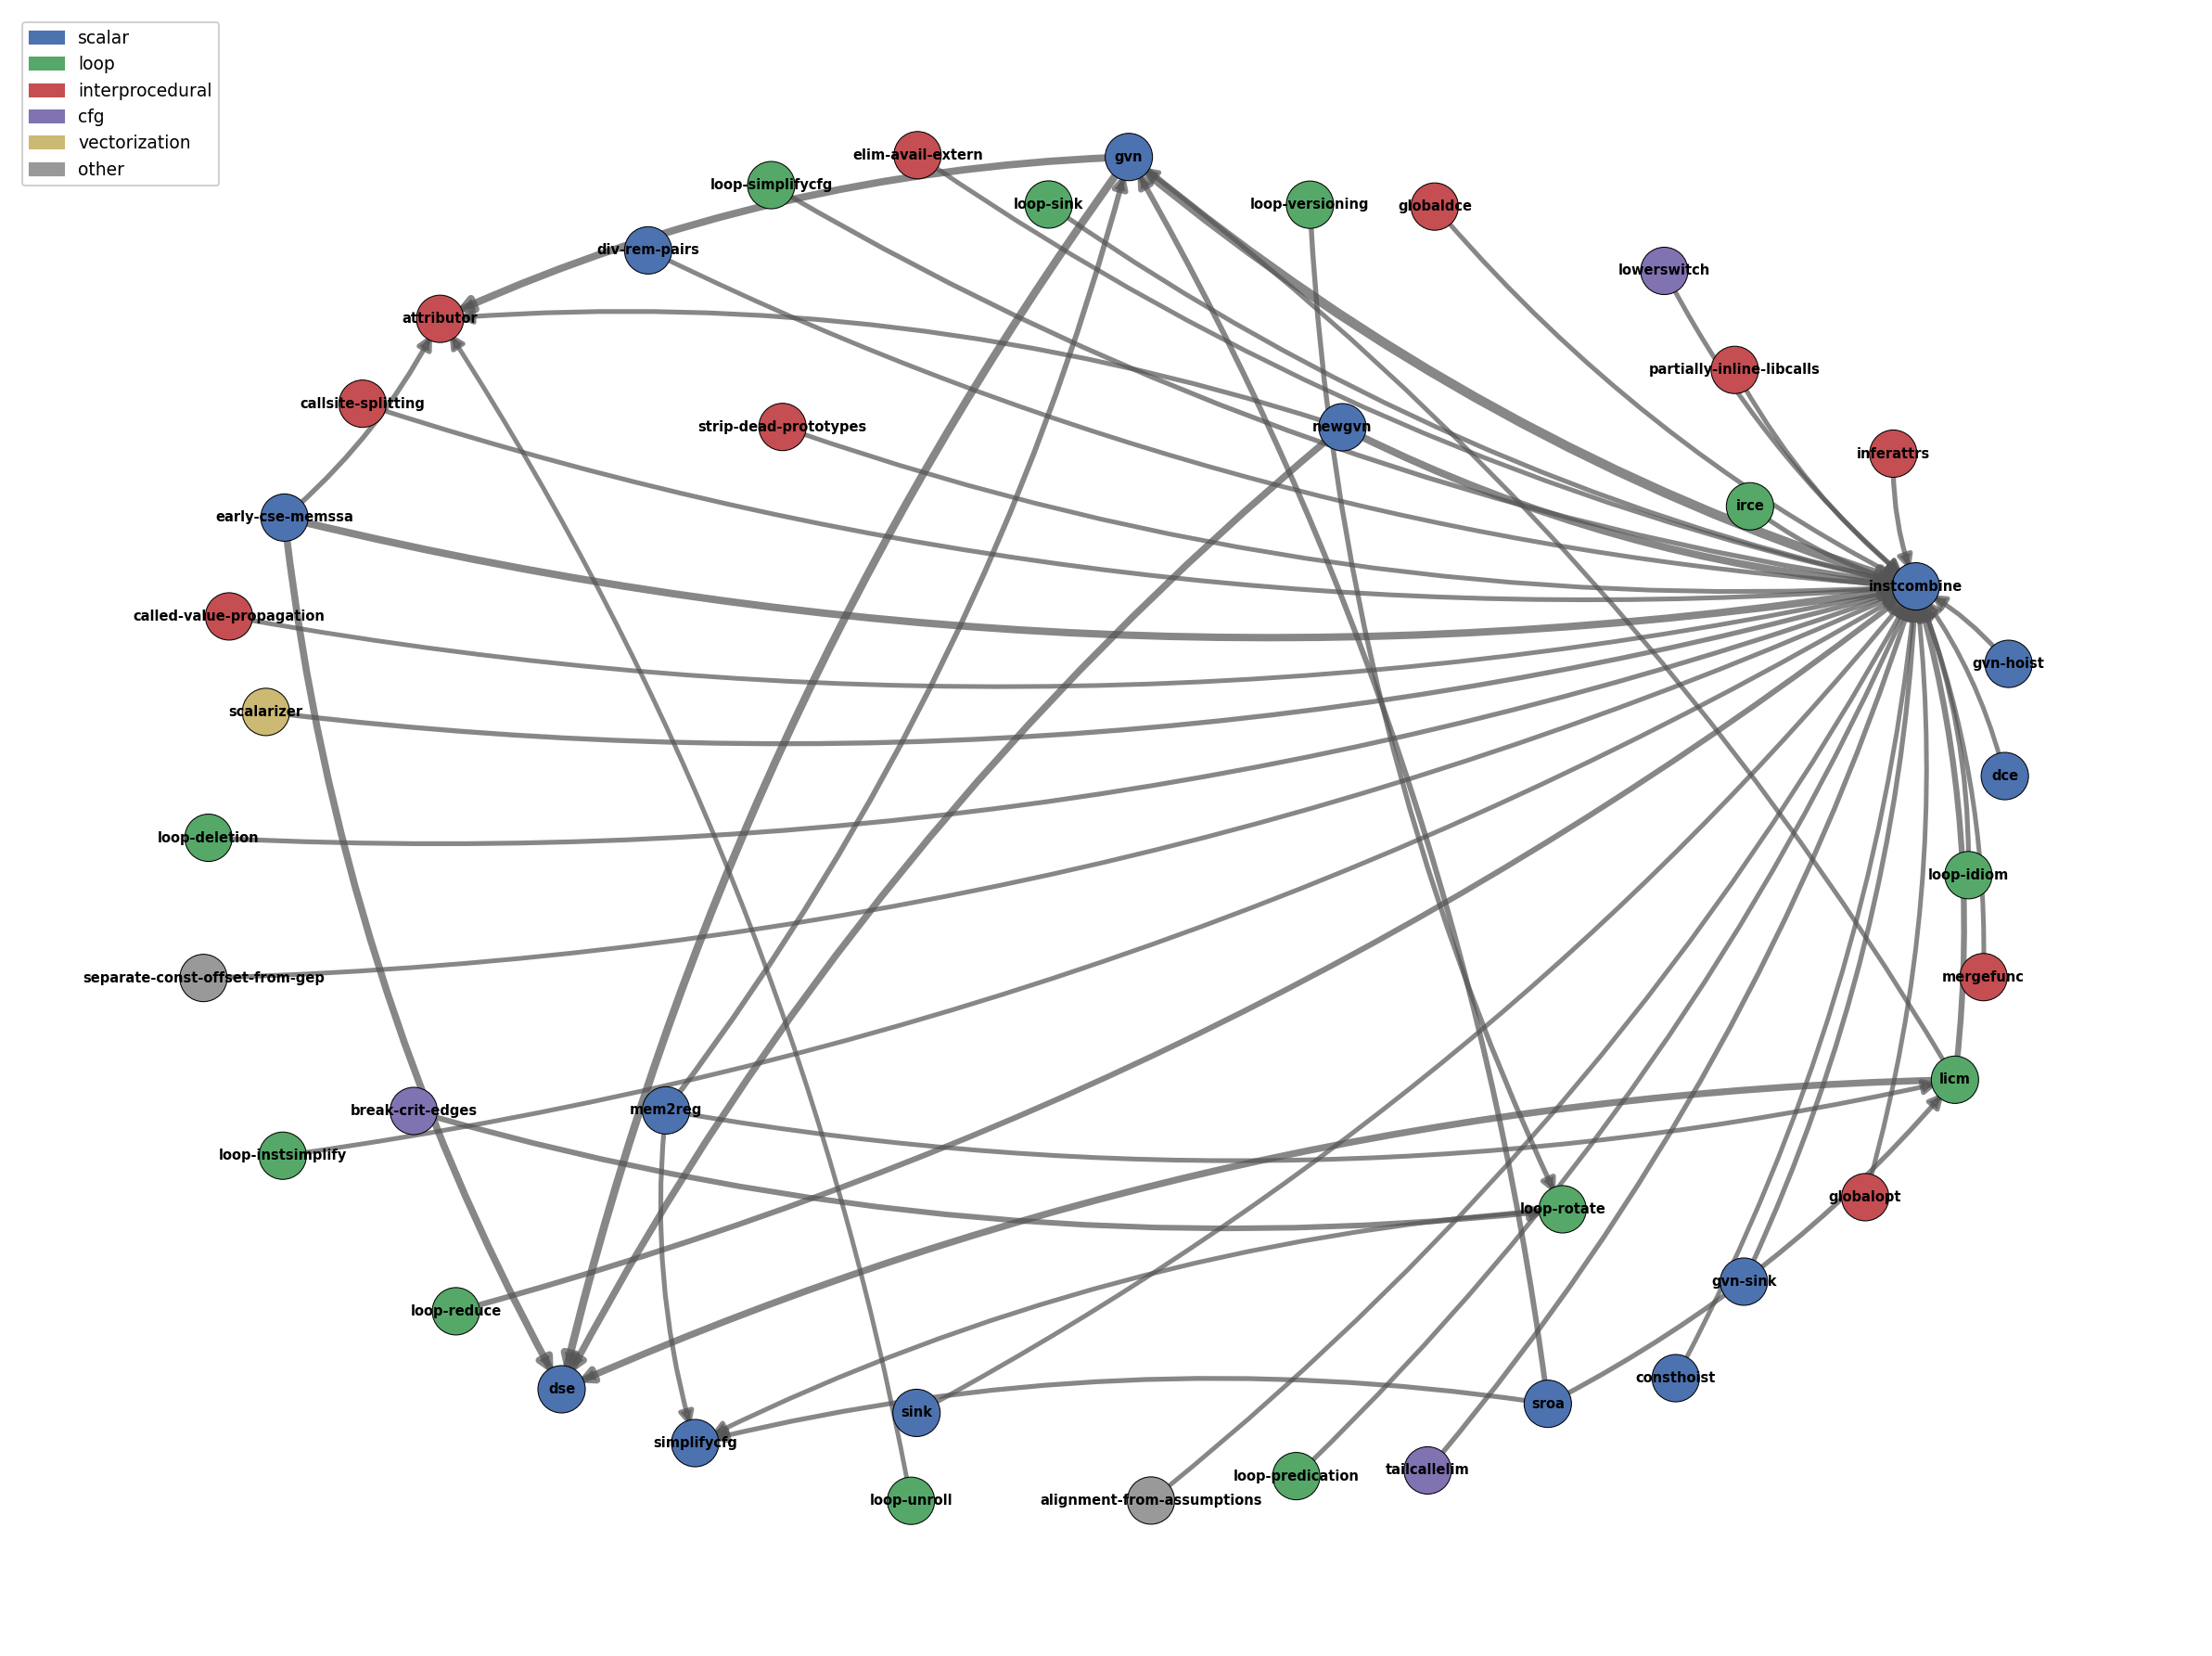
\includegraphics[width=\linewidth]{images/graph_global_top50_filtered.png}\\
      {\footnotesize Топ-50 рёбер содержательного графа.}
    \end{column}
    \begin{column}{0.4\textwidth}
      \small
      Доминирует паттерн \textbf{«вычисление значений $\to$ упрощение»}:
      \begin{itemize}\small
        \item источники~--- \texttt{gvn}, \texttt{newgvn}, \texttt{early-cse-memssa};
        \item стоки~--- \texttt{instcombine}, \texttt{dse}, \texttt{simplifycfg}.
      \end{itemize}
      \smallskip
      Рёбра \texttt{gvn}$\to$\texttt{instcombine} и \texttt{gvn}$\to$\texttt{dse}
      согласуются с реальным \texttt{-Oz}, где \texttt{gvn} стоит раньше обоих
      упрощающих проходов~--- \textbf{валидация метода}.
      \smallskip

      \texttt{-Oz} неоптимален: \textbf{374} из 517 программ имеют порядок лучше.
    \end{column}
  \end{columns}
\end{frame}

%% ================= Слайд 12: результат — каузальный vs корреляционный =================
\begin{frame}{Результат: каузальный граф $\ne$ корреляционный}
  \centering
  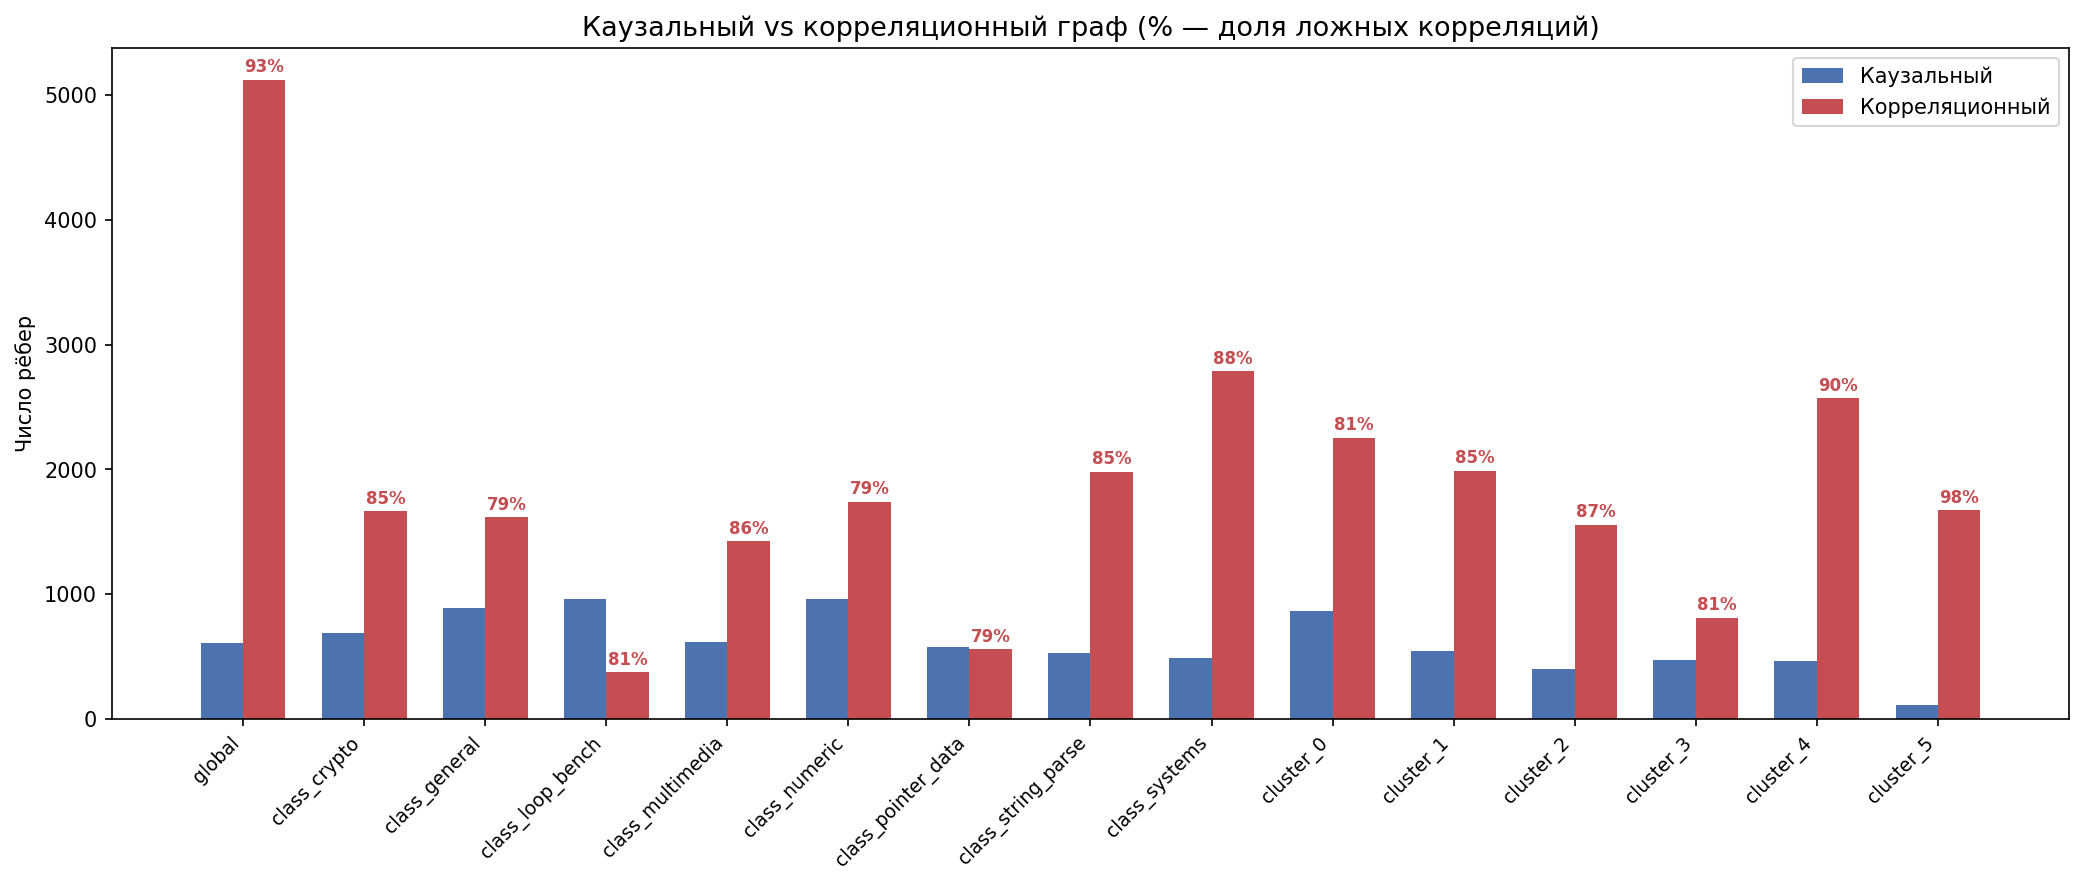
\includegraphics[width=0.9\linewidth]{images/comparison_causal_vs_corr.png}

  \smallskip
  \begin{columns}[c]
    \begin{column}{0.52\textwidth}
      \centering\small
      \begin{tabular}{@{}lr@{}}
        \toprule
        Каузальных рёбер      & \textbf{608}\\
        Корреляционных рёбер  & \textbf{5124}\\
        Пересечение           & 376\\
        \midrule
        \textbf{Доля ложных корреляций} & {\color{titlered}\textbf{92,7\,\%}}\\
        \bottomrule
      \end{tabular}
    \end{column}
    \begin{column}{0.48\textwidth}
      \small По 14 группам доля ложных корреляций составляет от \textbf{78,7\,\%}
      (general) до \textbf{98,1\,\%} (cluster\_5): большинство «значимых»
      корреляций между порядком пар и выигрышем \textbf{не имеют каузальной природы}.
    \end{column}
  \end{columns}
\end{frame}

%% ================= Слайд 13: результат — гетерогенность + формулировки =================
\begin{frame}{Результат: гетерогенность и две формулировки}
  \small
  \begin{columns}[T]
    \begin{column}{0.55\textwidth}
      \centering
      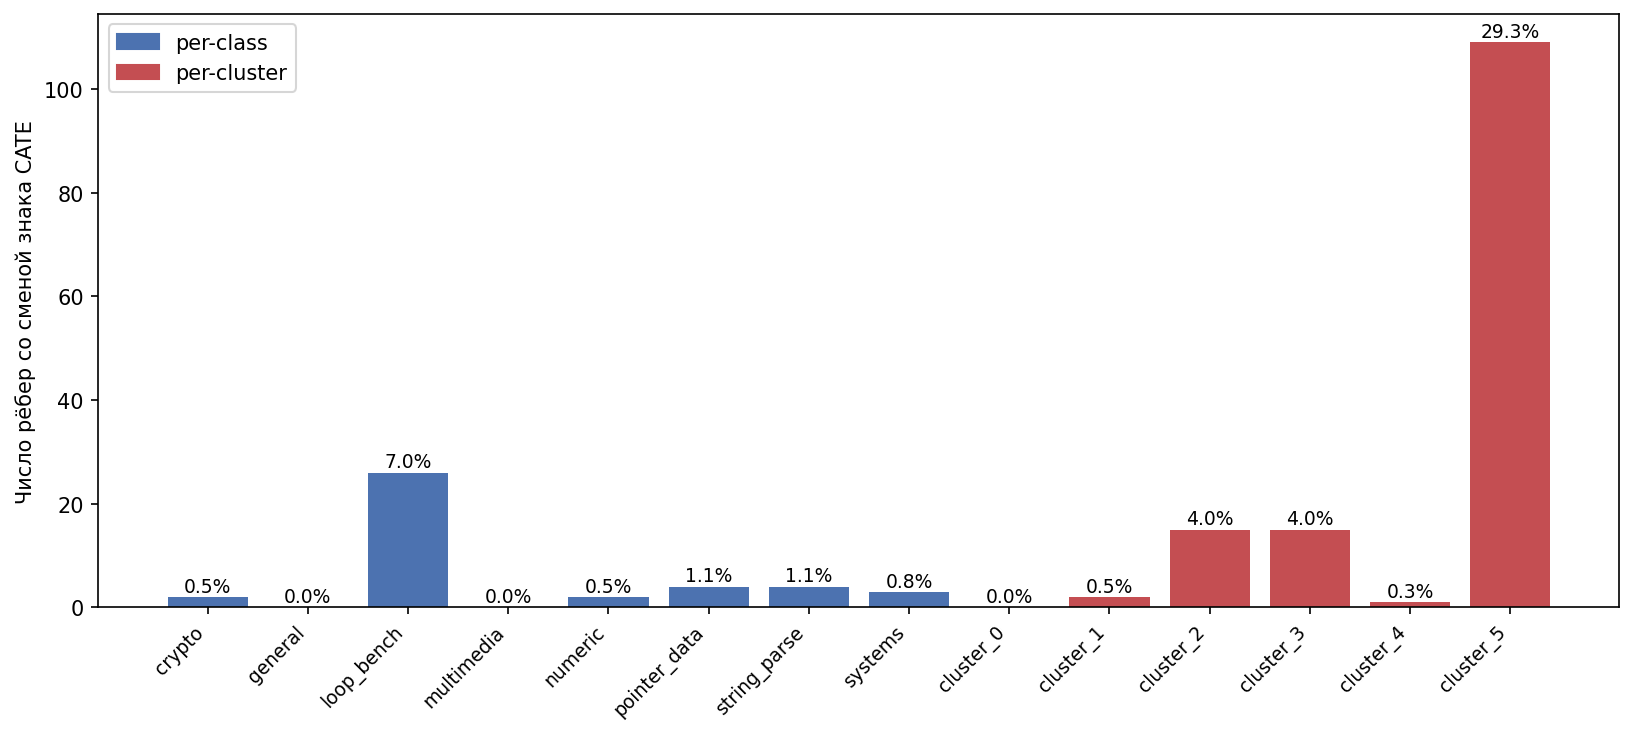
\includegraphics[width=\linewidth]{images/cate_flips_per_group.png}\\
      {\footnotesize Число рёбер, меняющих знак на подгруппе.}
    \end{column}
    \begin{column}{0.45\textwidth}
      \small
      \heading{Гетерогенность (CATE)}
      Эффект порядка \textbf{зависит от типа программы}: до \textbf{29\,\%} рёбер
      глобального графа меняют знак на отдельных кластерах. Универсального
      оптимального порядка не существует.

      \heading{Две формулировки}
      Относительный порядок даёт \textbf{608} рёбер (глобальные зависимости),
      соседство~--- \textbf{44} ребра (локальные синергии): формулировки выявляют
      \textbf{разные классы} зависимостей.
    \end{column}
  \end{columns}
\end{frame}

%% ================= Слайд 14: заключение — результаты =================
\begin{frame}{Заключение: основные результаты}
  Цель достигнута: построены интерпретируемые каузальные графы зависимостей
  между проходами LLVM. Ключевые численные результаты:
  \begin{enumerate}
    \item Метод оценки каузального эффекта порядка пар проходов \emph{без}
      алгоритмов поиска структуры (за счёт рандомизации).
    \item На собранных данных \textbf{92,7\,\%} статистически значимых корреляций
      «порядок--выигрыш» ложны (608 каузальных против 5124 корреляционных рёбер).
    \item Эффект порядка \textbf{гетерогенен}: до \textbf{29\,\%} рёбер меняют
      знак по кластерам программ.
    \item Две формулировки воздействия выявляют разные зависимости:
      \textbf{608} против \textbf{44} рёбер.
    \item Собраны датасеты: \textbf{517} программ в LLVM IR и \textbf{5,17 млн}
      прогонов с измеренной метрикой.
  \end{enumerate}
\end{frame}

%% ================= Слайд 15: положения на защиту =================
\begin{frame}{Положения, выносимые на защиту}
  \small
  \begin{enumerate}\setlength{\itemsep}{1pt}
    \item Случайные перестановки проходов LLVM образуют рандомизированный
      эксперимент, позволяющий оценивать каузальный эффект порядка пар напрямую,
      без алгоритмов поиска структуры.
    \item Предложен метод построения интерпретируемых каузальных графов
      зависимостей между проходами на нескольких уровнях агрегации.
    \item Значимая доля значимых корреляций между порядком проходов и улучшением
      метрики не имеет каузальной природы: каузальный и корреляционный графы
      существенно различаются.
    \item Эффект порядка гетерогенен по типам программ: для части зависимостей он
      меняет направление, единого оптимального порядка нет.
    \item Две формулировки воздействия (относительный порядок и соседство)
      выявляют разные классы зависимостей.
  \end{enumerate}

  \smallskip
  {\color{slideblue}\bfseries Значимость.} Основа для специализированных
  последовательностей под класс программ; развитие~--- генерация по графу.
\end{frame}

%% ================= Слайд 16: публикации =================
\begin{frame}{Публикации по теме работы}
  \begin{enumerate}
    \item \emph{Белонин~В.\,В., Ефанов~Н.\,Н.} Применение методов каузального
      вывода при анализе зависимостей между оптимизирующими проходами
      LLVM-компилятора~// 68-я Всероссийская научная конференция МФТИ.~--- 2026.
  \end{enumerate}
\end{frame}

\end{document}
